\documentclass[12pt,letterpaper]{article}\usepackage[]{graphicx}\usepackage[]{color}
%% maxwidth is the original width if it is less than linewidth
%% otherwise use linewidth (to make sure the graphics do not exceed the margin)
\makeatletter
\def\maxwidth{ %
  \ifdim\Gin@nat@width>\linewidth
    \linewidth
  \else
    \Gin@nat@width
  \fi
}
\makeatother

\definecolor{fgcolor}{rgb}{0.345, 0.345, 0.345}
\newcommand{\hlnum}[1]{\textcolor[rgb]{0.686,0.059,0.569}{#1}}%
\newcommand{\hlstr}[1]{\textcolor[rgb]{0.192,0.494,0.8}{#1}}%
\newcommand{\hlcom}[1]{\textcolor[rgb]{0.678,0.584,0.686}{\textit{#1}}}%
\newcommand{\hlopt}[1]{\textcolor[rgb]{0,0,0}{#1}}%
\newcommand{\hlstd}[1]{\textcolor[rgb]{0.345,0.345,0.345}{#1}}%
\newcommand{\hlkwa}[1]{\textcolor[rgb]{0.161,0.373,0.58}{\textbf{#1}}}%
\newcommand{\hlkwb}[1]{\textcolor[rgb]{0.69,0.353,0.396}{#1}}%
\newcommand{\hlkwc}[1]{\textcolor[rgb]{0.333,0.667,0.333}{#1}}%
\newcommand{\hlkwd}[1]{\textcolor[rgb]{0.737,0.353,0.396}{\textbf{#1}}}%

\usepackage{framed}
\makeatletter
\newenvironment{kframe}{%
 \def\at@end@of@kframe{}%
 \ifinner\ifhmode%
  \def\at@end@of@kframe{\end{minipage}}%
  \begin{minipage}{\columnwidth}%
 \fi\fi%
 \def\FrameCommand##1{\hskip\@totalleftmargin \hskip-\fboxsep
 \colorbox{shadecolor}{##1}\hskip-\fboxsep
     % There is no \\@totalrightmargin, so:
     \hskip-\linewidth \hskip-\@totalleftmargin \hskip\columnwidth}%
 \MakeFramed {\advance\hsize-\width
   \@totalleftmargin\z@ \linewidth\hsize
   \@setminipage}}%
 {\par\unskip\endMakeFramed%
 \at@end@of@kframe}
\makeatother

\definecolor{shadecolor}{rgb}{.97, .97, .97}
\definecolor{messagecolor}{rgb}{0, 0, 0}
\definecolor{warningcolor}{rgb}{1, 0, 1}
\definecolor{errorcolor}{rgb}{1, 0, 0}
\newenvironment{knitrout}{}{} % an empty environment to be redefined in TeX

\usepackage{alltt}
\usepackage[utf8]{inputenc}
\usepackage[margin=.7in]{geometry}
\usepackage{graphicx}
\usepackage{titling}
\usepackage{amsmath}
\usepackage{amsfonts}
\usepackage{amssymb}
\renewcommand{\theenumiv}{\arabic{enumiv}}
\setlength{\droptitle}{-5em}
\author{Maurice Diesendruck\vspace{-2ex}}
\title{StatMod2 - Hierarchical Models and Shrinkage - Exercises 4\vspace{-1ex}}
\IfFileExists{upquote.sty}{\usepackage{upquote}}{}
\begin{document}
\maketitle

\section{School Averages and Sample Size}

Larger samples tend to "smooth" out extreme scores, so small samples are more 
likely to be extreme.\\

\begin{knitrout}
\definecolor{shadecolor}{rgb}{0.969, 0.969, 0.969}\color{fgcolor}\begin{kframe}
\begin{alltt}
\hlstd{data} \hlkwb{<-} \hlkwd{read.csv}\hlstd{(}\hlstr{"mathtest.csv"}\hlstd{)}
\hlkwd{attach}\hlstd{(data)}
\hlkwd{boxplot}\hlstd{(mathscore} \hlopt{~} \hlstd{school,} \hlkwc{xlab}\hlstd{=}\hlstr{"School"}\hlstd{,} \hlkwc{ylab}\hlstd{=}\hlstr{"Score"}\hlstd{)}
\end{alltt}
\end{kframe}
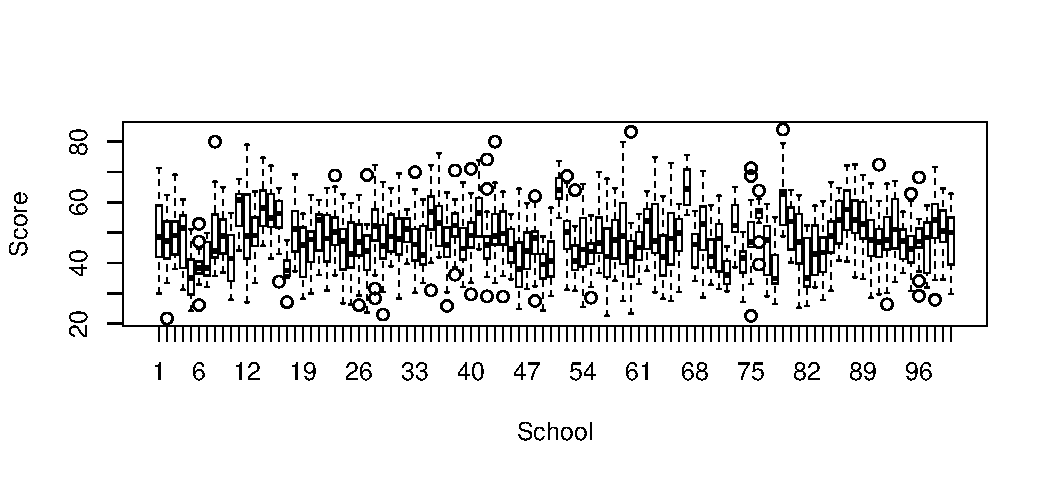
\includegraphics[width=\maxwidth]{figure/unnamed-chunk-1-1} 
\begin{kframe}\begin{alltt}
\hlstd{school.avgs} \hlkwb{<-} \hlkwd{aggregate}\hlstd{(data,} \hlkwd{list}\hlstd{(}\hlkwc{school}\hlstd{=school), mean)[,}\hlnum{3}\hlstd{]}
\hlstd{school.ssize} \hlkwb{<-} \hlkwd{aggregate}\hlstd{(data,} \hlkwd{list}\hlstd{(}\hlkwc{school}\hlstd{=school), length)[,}\hlnum{3}\hlstd{]}
\hlkwd{plot}\hlstd{(}\hlkwd{cbind}\hlstd{(school.avgs, school.ssize))}
\hlstd{fit} \hlkwb{<-} \hlkwd{lowess}\hlstd{(}\hlkwd{cbind}\hlstd{(school.avgs, school.ssize))}
\hlkwd{lines}\hlstd{(fit)}
\end{alltt}
\end{kframe}
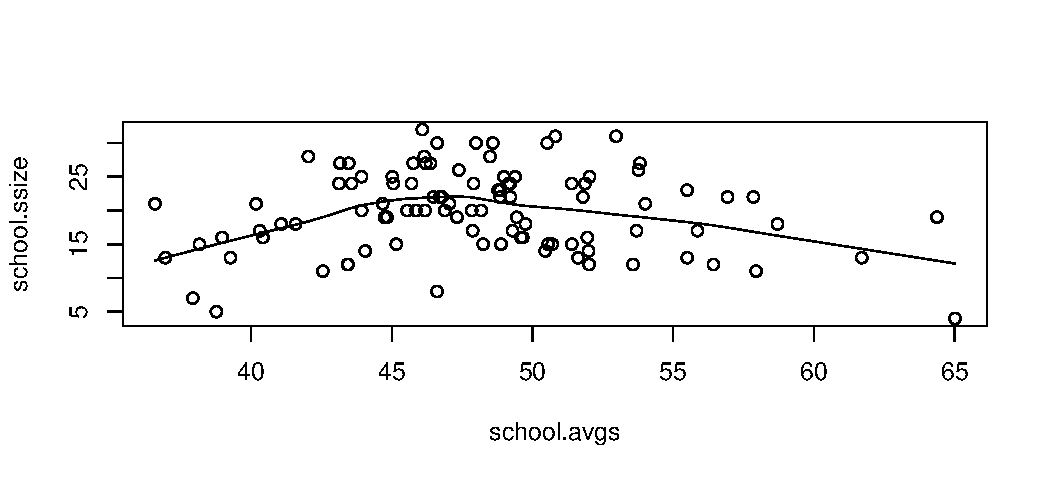
\includegraphics[width=\maxwidth]{figure/unnamed-chunk-1-2} 

\end{knitrout}

\subsection{Normal Hierarchical Model with Gibbs Sampling}

\subsubsection{Model}
For school $i=1,\cdots,p$; student $j=1,\cdots,n_i$; and $\sum n_i = n$; 
let $a=b=c=d=1$, and note that for this data, $p=100$ and $n=1993$:
\begin{align*}
  y_{ij} &\sim\ N(\theta_i,\sigma^2)\\
  \theta_i &\sim\ N(\mu,\tau^2)\\
  \mu &\sim\ N(m, v)\\
  \sigma^2 &\sim\ InvGa(a,b)\\
  \tau^2 &\sim\ InvGa(c,d)\\
\end{align*}

\subsubsection{Joint and Posterior Distributions}

See attached sheets.

\subsubsection{Gibbs Sampler}

The Gibbs Sampler produces the following results. Immediately below are the posterior estimates for $\theta$.

\begin{knitrout}
\definecolor{shadecolor}{rgb}{0.969, 0.969, 0.969}\color{fgcolor}\begin{kframe}
\begin{verbatim}
##   [1] 50.58284 46.71190 48.64918 47.53231 38.42593 40.80959 41.86254
##   [8] 48.81365 49.07595 42.37583 55.31309 50.25993 49.24975 56.87413
##  [15] 54.18940 54.40644 41.43114 49.99969 44.59810 46.21529 50.21534
##  [22] 47.99002 51.15485 45.94356 45.39898 46.85521 44.57778 51.39281
##  [29] 46.58123 49.26433 49.08094 50.08204 47.42765 46.10978 54.47988
##  [36] 52.15082 46.29173 51.17746 46.44004 48.83534 55.67513 46.45156
##  [43] 50.82646 49.06740 45.78828 41.32091 44.46692 47.04440 40.15568
##  [50] 42.66953 61.58872 49.16084 43.98694 46.62612 43.78124 49.08188
##  [57] 44.51959 48.43275 49.37334 42.70601 45.48414 50.79106 49.27863
##  [64] 43.77570 47.91054 48.17478 56.84499 45.36645 51.46214 44.15908
##  [71] 46.90269 39.51138 53.01305 41.79331 48.72754 53.82094 45.29305
##  [78] 41.21583 58.57092 51.24315 47.04516 42.92000 44.90826 44.25397
##  [85] 48.59957 52.65977 56.31267 53.11828 53.12795 48.52563 47.86088
##  [92] 48.25425 51.55690 47.03614 45.49883 47.19830 46.02330 52.44622
##  [99] 50.95304 48.01554
\end{verbatim}
\end{kframe}
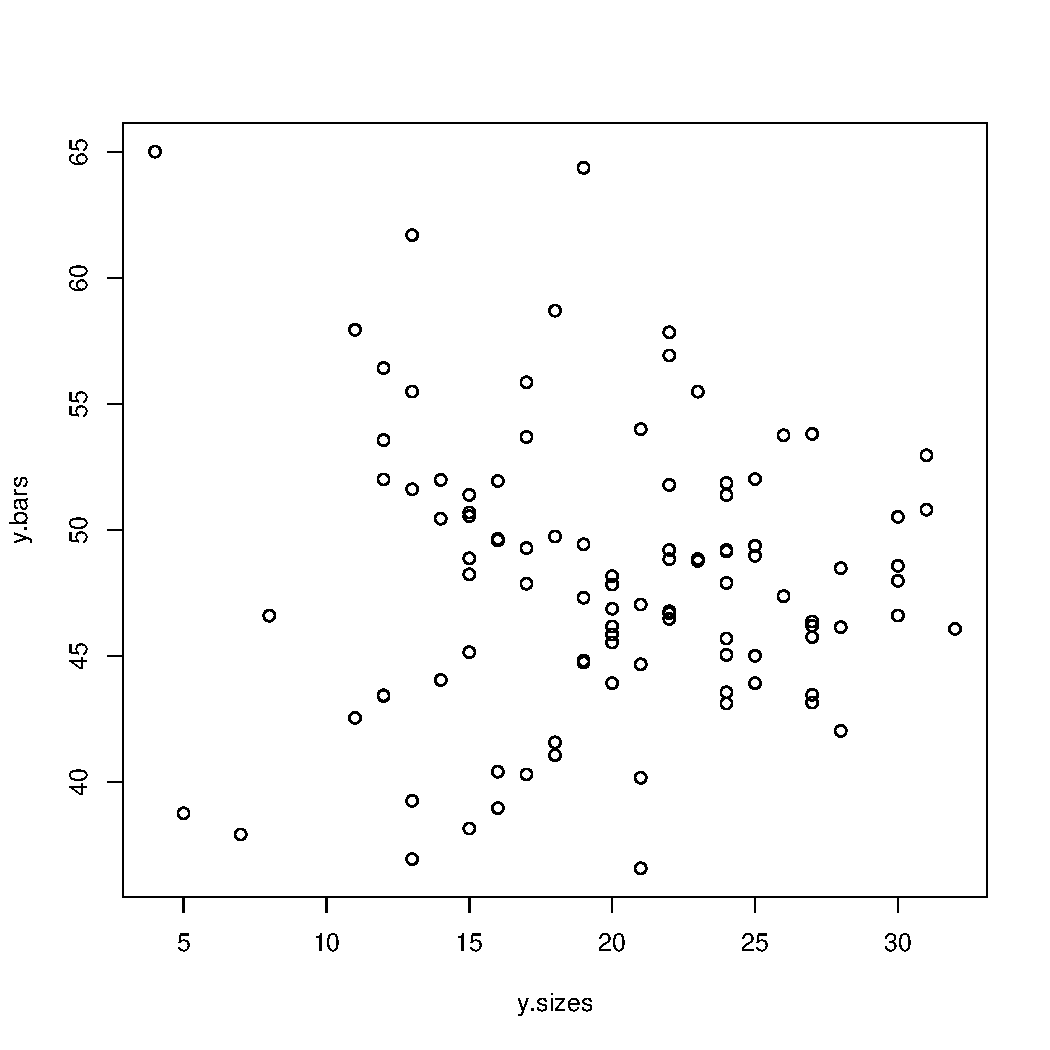
\includegraphics[width=\maxwidth]{figure/unnamed-chunk-2-1} 

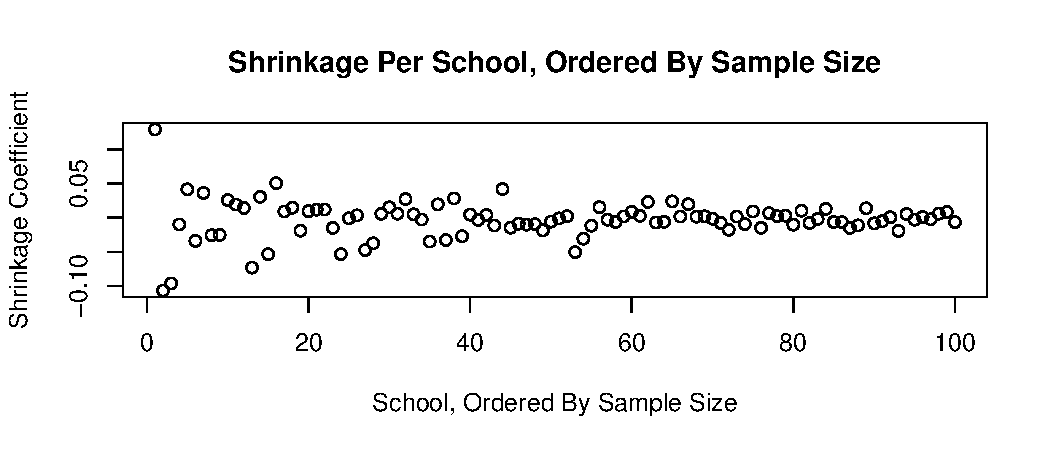
\includegraphics[width=\maxwidth]{figure/unnamed-chunk-2-2} 

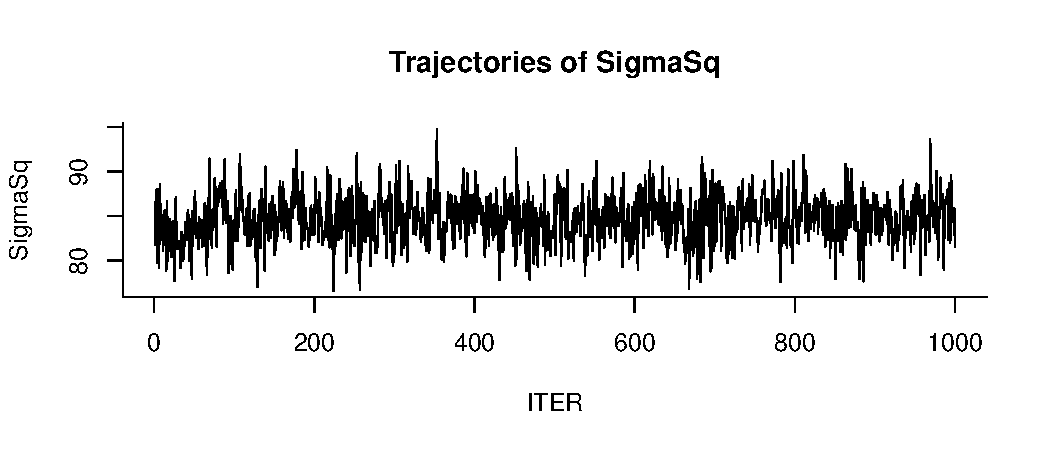
\includegraphics[width=\maxwidth]{figure/unnamed-chunk-2-3} 

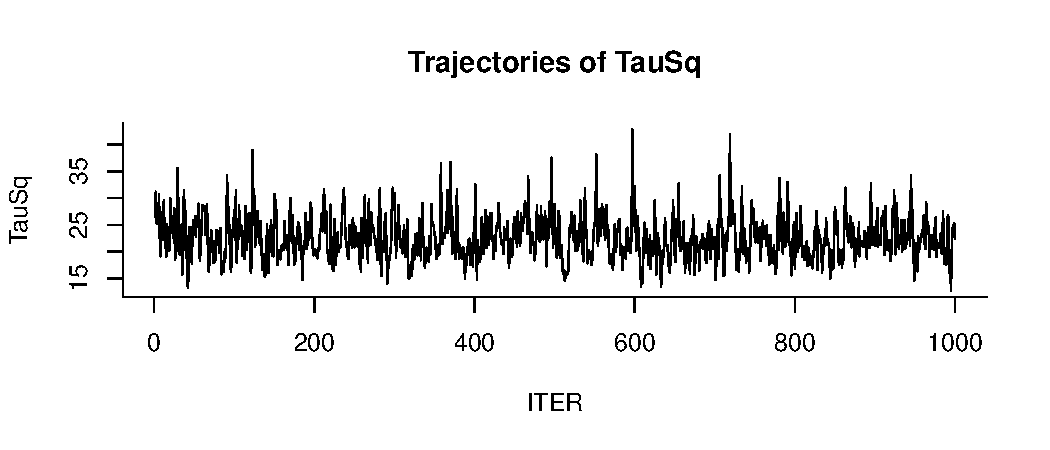
\includegraphics[width=\maxwidth]{figure/unnamed-chunk-2-4} 

\end{knitrout}

\subsection{Shrinkage}

In general, the smaller the sample size, the more extreme the sample mean, and the larger the shrinkage coefficient. 

\end{document}

